\documentclass[tikz]{standalone}
\usetikzlibrary{shapes,arrows.meta}
\begin{document}
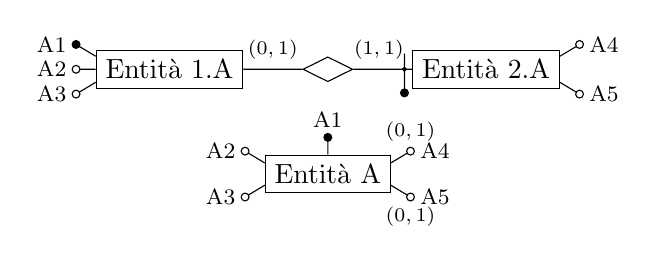
\begin{tikzpicture}
    \draw

    %%* Attributi:
    %%  node[draw, circle, inner sep=1pt,anchor=180, fill=black]{}node[right]{\footnotesize A}
    %%? Distanza orizzontale: E -(0.25,0.x)- A
    %%? Distanza verticale: E -(0,x * 0.22)- A

    %%* Cardinalità:
    %%  node[below right]{\scriptsize $(0,N)$}
    %%  node[above right]{\scriptsize $(0,N)$}
    %%  node[midway, above]{\scriptsize $(0,N)$}

    %%* Relazione:
    %%  node[draw, diamond, shape aspect=2, inner sep=3pt, anchor=90](r1){}
    %%  node[draw, diamond, shape aspect=2, inner sep=0.2pt, anchor=180](r2){R2}

    %%* Entità:
    %%  node[draw, rectangle, anchor=90](e1){}
    %%? Distanza verticale: E -(0.3)- R -(0.3) E
    %%? Distanza orizzontale: E -(0.75)- R -(0.75)- E

    %%* Entità 1
    (0,-1.5)node[draw, rectangle, anchor=180](e1){Entità 1.A}
    (e1.170)--++(-0.25,.15)node[draw, circle, inner sep=1pt, fill=black]{}node[left]{\footnotesize A1}
    (e1.180)--++(-0.25,0)  node[draw, circle, inner sep=1pt, fill=white]{}node[left]{\footnotesize A2}
    (e1.190)--++(-.25,-.15)node[draw, circle, inner sep=1pt, fill=white]{}node[left]{\footnotesize A3}

    %%* Relationship
    (e1.0)--++(0.75,0)node[midway, above]{\scriptsize $(0,1)$}node[draw, diamond, shape aspect=2, inner sep=3pt, anchor=180](r1){}

    
    (r1.90)++(0,-1.25)node[draw, rectangle, anchor=90](e0){Entità A}
    (e0.170)--++(-0.25,.15)node[draw, circle, inner sep=1pt, fill=white]{}node[left]{\footnotesize A2}
    (e0.190)--++(-.25,-.15)node[draw, circle, inner sep=1pt, fill=white]{}node[left]{\footnotesize A3}
    (e0.90)--++(0,0.22)node[draw, circle, inner sep=1pt, fill=black]{}node[above]{\footnotesize A1}
    (e0.10)--++(.25,.15)node[draw, circle, inner sep=1pt, fill=white]{}node[right]{\footnotesize A4}node[above]{\scriptsize $(0,1)$}
    (e0.350)--++(.25,-.15)node[draw, circle, inner sep=1pt, fill=white]{}node[right]{\footnotesize A5}node[below]{\scriptsize $(0,1)$}

    %%* Entità 2
    (r1.0)--++(0.65,0)node[midway, above]{\scriptsize $(1,1)$}node[draw, circle, inner sep=0.5pt, fill=black](a){}--++(0.1,0)node[draw, rectangle, anchor=180](e2){Entità 2.A}
    (e2.10)--++(.25,.15)node[draw, circle, inner sep=1pt, fill=white]{}node[right]{\footnotesize A4}
    (e2.350)--++(.25,-.15)node[draw, circle, inner sep=1pt, fill=white]{}node[right]{\footnotesize A5}

    (a)++(0,0.2)--++(0,-0.5)node[draw, circle, inner sep=1pt, fill=black]{}
    ;
\end{tikzpicture}
\end{document}